%cant fit it....
\section{システムのモデリング}
本章では,提案する不安定物体を支持可能な群ロボットシステムとシステムのモデリングについて説明する.
提案システムを実現するために,ロボット群が物体を支持する支持部とシステム全体を移動する移動部に分ける必要がある.
また,ロボットの台数は限られているので,支持部のロボットの台数が多いほど,物体を安定に支持できるが,移動部に負担がかかるため,全体の移動速度が遅くなることが考えられる.一方,移動部に関しては,ロボットが多いほど,全体の速度は速いが,支持部のロボットが少ないため,物体が倒れる可能性がある.
本稿ではその前段階として,支持部のロボットが物体を支えるための条件を検討する.

提案システムのモデリングした図を\reffig{modeling}に示す.
\begin{figure}[b]
  \centering
  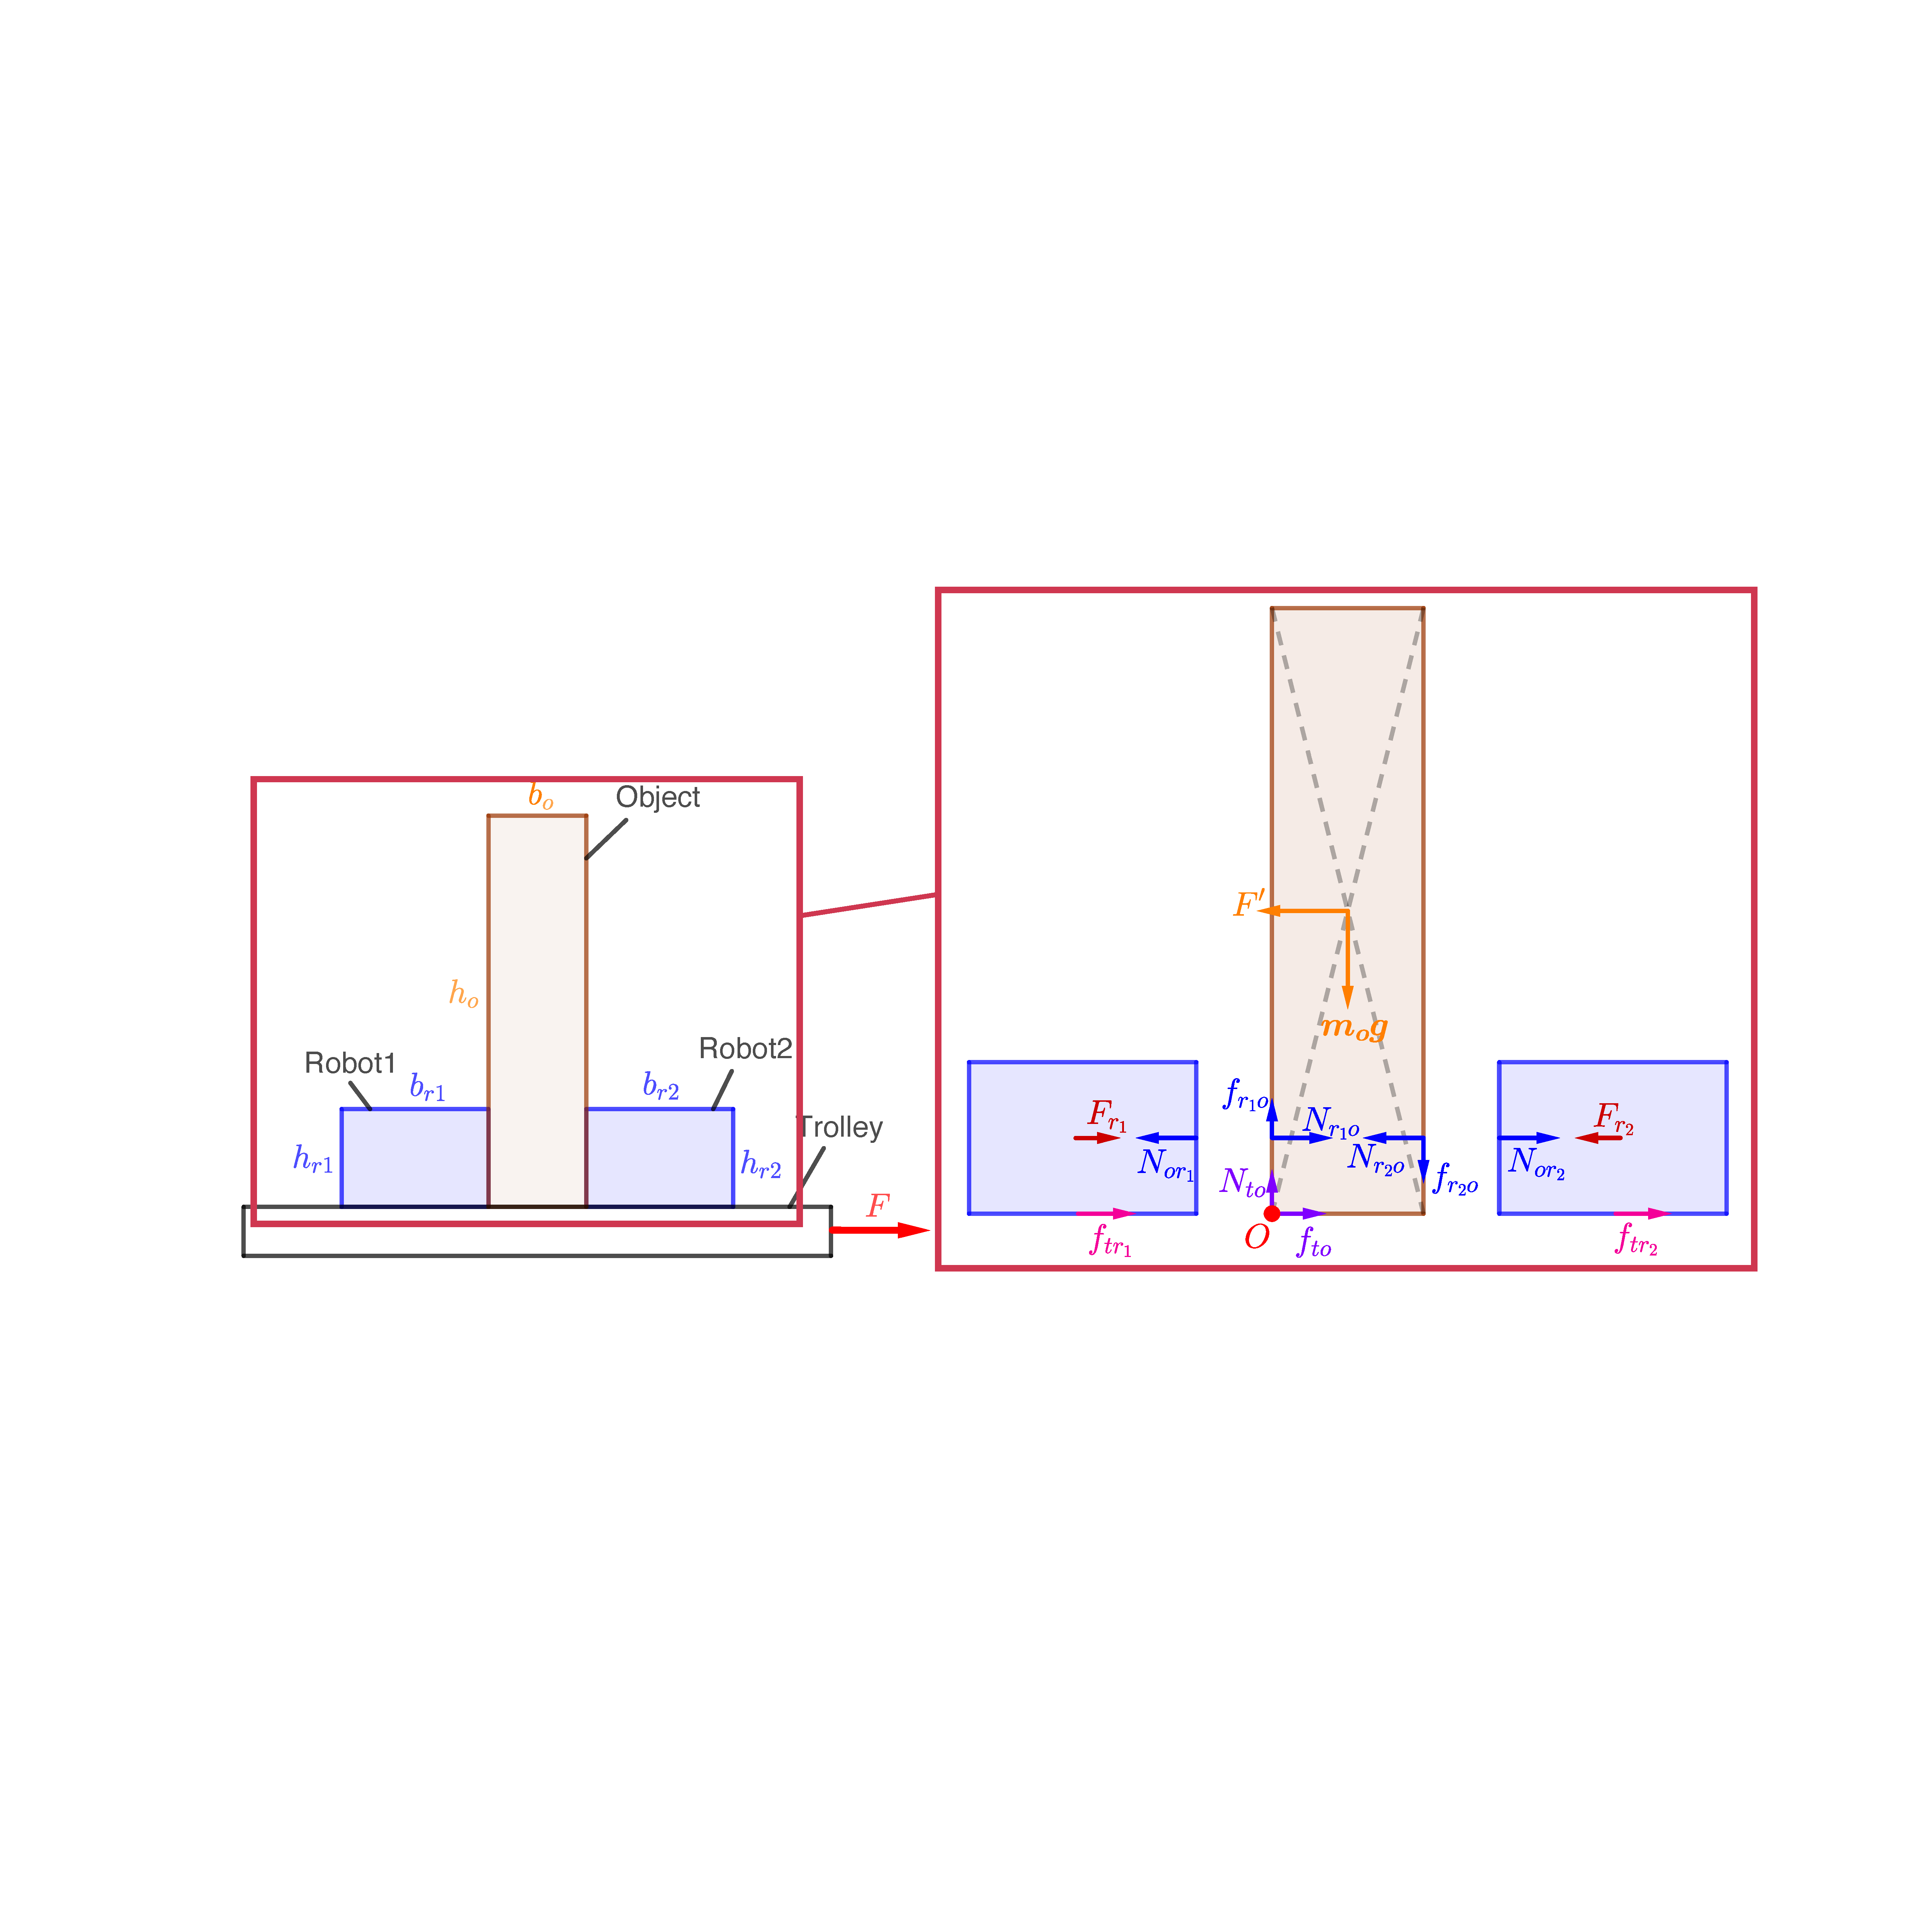
\includegraphics[width=0.9\columnwidth]{figures/modeling.pdf}
  \caption{Simplified model, free body diagram}
  \label{fig:modeling}
\end{figure}
また,モデリングに使用した変数を\reftab{model-parameter}に示す.
\begin{table}[tb]
\caption{Parameters of model}
\centering
\scalebox{0.7}{
\begin{tabular}{c|c}
\hline
Parameter & Description                   \\ \hline\hline
$b_o$       & Width of object              \\ \hline
$h_o$      & Height of object               \\ \hline
$h_r$      & Height of robot               \\ \hline
$m_o$     & Mass of object        \\ \hline
$f_{r_1 o}$       & Friction from robot1 acting on object                 \\ \hline
$f_{r_2 o}$ & Friction from robot2 acting on object                 \\ \hline
$f_{t o}$ & Friction from trolley acting on object                 \\ \hline
$N_{t o}$ & Normal force from trolley acting on object                 \\ \hline
$N_{r_1 o}$ & Normal force from robot1 acting on object                 \\ \hline
$N_{r_2 o}$ & Normal force from robot2 acting on object                 \\ \hline
$F_{r_1}$ & Force asserted by robot1                 \\ \hline
$F_{r_2}$ & Force asserted by robot2                 \\ \hline
\end{tabular}}
\label{tab:model-parameter}
\end{table}
次に,台車に大きな力$F$がかかっても物体は傾かないための条件を調べる.
点$O$まわりのモーメントの釣り合いから,以下の式が導かれる.
\[
    F<\frac{h_{r}}{h_{o}}\left(F_{r_{1}}-F_{r_{2}}+f_{t{r_1}}+f_{t{r_2}}\right)+\frac{b_{o}}{h_{o}}\left(m_{o} g+2 f_{r_2 o}\right)
\]
上式より,右辺を大きくすることで,物体をより安定に運べる.
今回,ロボットと台車の間の摩擦$f_{t{r_1}},f_{t{r_2}}$を大きくすることとロボットに前進力$F_{r_{1}},F_{r_{2}}$をかけることに注目した.